\documentclass[]{article}
\usepackage{lmodern}
\usepackage{amssymb,amsmath}
\usepackage{ifxetex,ifluatex}
\usepackage{fixltx2e} % provides \textsubscript
\ifnum 0\ifxetex 1\fi\ifluatex 1\fi=0 % if pdftex
  \usepackage[T1]{fontenc}
  \usepackage[utf8]{inputenc}
\else % if luatex or xelatex
  \ifxetex
    \usepackage{mathspec}
  \else
    \usepackage{fontspec}
  \fi
  \defaultfontfeatures{Ligatures=TeX,Scale=MatchLowercase}
\fi
% use upquote if available, for straight quotes in verbatim environments
\IfFileExists{upquote.sty}{\usepackage{upquote}}{}
% use microtype if available
\IfFileExists{microtype.sty}{%
\usepackage{microtype}
\UseMicrotypeSet[protrusion]{basicmath} % disable protrusion for tt fonts
}{}
\usepackage[margin=1in]{geometry}
\usepackage{hyperref}
\hypersetup{unicode=true,
            pdftitle={Markov models for cost-effectiveness analysis in R},
            pdfauthor={Fernando Alarid-Escudero, PhD; Eric Jutkowitz, PhD; Karen M. Kuntz, ScD\^{}*},
            pdfborder={0 0 0},
            breaklinks=true}
\urlstyle{same}  % don't use monospace font for urls
\usepackage{color}
\usepackage{fancyvrb}
\newcommand{\VerbBar}{|}
\newcommand{\VERB}{\Verb[commandchars=\\\{\}]}
\DefineVerbatimEnvironment{Highlighting}{Verbatim}{commandchars=\\\{\}}
% Add ',fontsize=\small' for more characters per line
\usepackage{framed}
\definecolor{shadecolor}{RGB}{248,248,248}
\newenvironment{Shaded}{\begin{snugshade}}{\end{snugshade}}
\newcommand{\KeywordTok}[1]{\textcolor[rgb]{0.13,0.29,0.53}{\textbf{#1}}}
\newcommand{\DataTypeTok}[1]{\textcolor[rgb]{0.13,0.29,0.53}{#1}}
\newcommand{\DecValTok}[1]{\textcolor[rgb]{0.00,0.00,0.81}{#1}}
\newcommand{\BaseNTok}[1]{\textcolor[rgb]{0.00,0.00,0.81}{#1}}
\newcommand{\FloatTok}[1]{\textcolor[rgb]{0.00,0.00,0.81}{#1}}
\newcommand{\ConstantTok}[1]{\textcolor[rgb]{0.00,0.00,0.00}{#1}}
\newcommand{\CharTok}[1]{\textcolor[rgb]{0.31,0.60,0.02}{#1}}
\newcommand{\SpecialCharTok}[1]{\textcolor[rgb]{0.00,0.00,0.00}{#1}}
\newcommand{\StringTok}[1]{\textcolor[rgb]{0.31,0.60,0.02}{#1}}
\newcommand{\VerbatimStringTok}[1]{\textcolor[rgb]{0.31,0.60,0.02}{#1}}
\newcommand{\SpecialStringTok}[1]{\textcolor[rgb]{0.31,0.60,0.02}{#1}}
\newcommand{\ImportTok}[1]{#1}
\newcommand{\CommentTok}[1]{\textcolor[rgb]{0.56,0.35,0.01}{\textit{#1}}}
\newcommand{\DocumentationTok}[1]{\textcolor[rgb]{0.56,0.35,0.01}{\textbf{\textit{#1}}}}
\newcommand{\AnnotationTok}[1]{\textcolor[rgb]{0.56,0.35,0.01}{\textbf{\textit{#1}}}}
\newcommand{\CommentVarTok}[1]{\textcolor[rgb]{0.56,0.35,0.01}{\textbf{\textit{#1}}}}
\newcommand{\OtherTok}[1]{\textcolor[rgb]{0.56,0.35,0.01}{#1}}
\newcommand{\FunctionTok}[1]{\textcolor[rgb]{0.00,0.00,0.00}{#1}}
\newcommand{\VariableTok}[1]{\textcolor[rgb]{0.00,0.00,0.00}{#1}}
\newcommand{\ControlFlowTok}[1]{\textcolor[rgb]{0.13,0.29,0.53}{\textbf{#1}}}
\newcommand{\OperatorTok}[1]{\textcolor[rgb]{0.81,0.36,0.00}{\textbf{#1}}}
\newcommand{\BuiltInTok}[1]{#1}
\newcommand{\ExtensionTok}[1]{#1}
\newcommand{\PreprocessorTok}[1]{\textcolor[rgb]{0.56,0.35,0.01}{\textit{#1}}}
\newcommand{\AttributeTok}[1]{\textcolor[rgb]{0.77,0.63,0.00}{#1}}
\newcommand{\RegionMarkerTok}[1]{#1}
\newcommand{\InformationTok}[1]{\textcolor[rgb]{0.56,0.35,0.01}{\textbf{\textit{#1}}}}
\newcommand{\WarningTok}[1]{\textcolor[rgb]{0.56,0.35,0.01}{\textbf{\textit{#1}}}}
\newcommand{\AlertTok}[1]{\textcolor[rgb]{0.94,0.16,0.16}{#1}}
\newcommand{\ErrorTok}[1]{\textcolor[rgb]{0.64,0.00,0.00}{\textbf{#1}}}
\newcommand{\NormalTok}[1]{#1}
\usepackage{longtable,booktabs}
\usepackage{graphicx,grffile}
\makeatletter
\def\maxwidth{\ifdim\Gin@nat@width>\linewidth\linewidth\else\Gin@nat@width\fi}
\def\maxheight{\ifdim\Gin@nat@height>\textheight\textheight\else\Gin@nat@height\fi}
\makeatother
% Scale images if necessary, so that they will not overflow the page
% margins by default, and it is still possible to overwrite the defaults
% using explicit options in \includegraphics[width, height, ...]{}
\setkeys{Gin}{width=\maxwidth,height=\maxheight,keepaspectratio}
\IfFileExists{parskip.sty}{%
\usepackage{parskip}
}{% else
\setlength{\parindent}{0pt}
\setlength{\parskip}{6pt plus 2pt minus 1pt}
}
\setlength{\emergencystretch}{3em}  % prevent overfull lines
\providecommand{\tightlist}{%
  \setlength{\itemsep}{0pt}\setlength{\parskip}{0pt}}
\setcounter{secnumdepth}{5}
% Redefines (sub)paragraphs to behave more like sections
\ifx\paragraph\undefined\else
\let\oldparagraph\paragraph
\renewcommand{\paragraph}[1]{\oldparagraph{#1}\mbox{}}
\fi
\ifx\subparagraph\undefined\else
\let\oldsubparagraph\subparagraph
\renewcommand{\subparagraph}[1]{\oldsubparagraph{#1}\mbox{}}
\fi

%%% Use protect on footnotes to avoid problems with footnotes in titles
\let\rmarkdownfootnote\footnote%
\def\footnote{\protect\rmarkdownfootnote}

%%% Change title format to be more compact
\usepackage{titling}

% Create subtitle command for use in maketitle
\newcommand{\subtitle}[1]{
  \posttitle{
    \begin{center}\large#1\end{center}
    }
}

\setlength{\droptitle}{-2em}
  \title{Markov models for cost-effectiveness analysis in R}
  \pretitle{\vspace{\droptitle}\centering\huge}
  \posttitle{\par}
  \author{Fernando Alarid-Escudero, PhD\footnote{Division of Health Policy and
  Management, University of Minnesota School of Public Health,
  Minneapolis, MN, USA} \\ Eric Jutkowitz, PhD\footnote{Department of Health Services, Policy and
  Practice, Brown University School of Public Health, Providence, RI,
  USA} \\ Karen M. Kuntz, ScD\(^*\)}
  \preauthor{\centering\large\emph}
  \postauthor{\par}
  \predate{\centering\large\emph}
  \postdate{\par}
  \date{2018-02-03}

\usepackage{booktabs}
\usepackage{longtable}
\usepackage{array}
\usepackage{multirow}
\usepackage[table]{xcolor}
\usepackage{wrapfig}
\usepackage{float}
\usepackage{colortbl}
\usepackage{pdflscape}
\usepackage{tabu}
\usepackage{threeparttable}

\usepackage{amsthm}
\newtheorem{theorem}{Theorem}[section]
\newtheorem{lemma}{Lemma}[section]
\theoremstyle{definition}
\newtheorem{definition}{Definition}[section]
\newtheorem{corollary}{Corollary}[section]
\newtheorem{proposition}{Proposition}[section]
\theoremstyle{definition}
\newtheorem{example}{Example}[section]
\theoremstyle{definition}
\newtheorem{exercise}{Exercise}[section]
\theoremstyle{remark}
\newtheorem*{remark}{Remark}
\newtheorem*{solution}{Solution}
\begin{document}
\maketitle

{
\setcounter{tocdepth}{4}
\tableofcontents
}
This document shows an example of how to conduct decision-analytic
models in R (Jalal et al. \protect\hyperlink{ref-Jalal2017b}{2017})
using the R package \texttt{dampack}.

The R package \texttt{dampack} has a couple functions that could be used
to evaluate Markov models. Specifically, the function
\texttt{CalculateMarkovTrace} takes a transition probability matrix
(time-homogeneous) or array (time-dependent) and then simulates a cohort
of hypothetical individuals, and returns a cohort trace and transition
array. The function \texttt{ExpectedValue} takes a transition array and
rewards matrix, and calculates expected outcomes. The package can be
used to compare competing strategies and calculate their
cost-effectiveness. Below, we provide an applied example of these
functions.

\section{Model Description}\label{model-description}

We will develop a 4-state Markov model to quantify the expected outcomes
for a cohort of 55-year-old women who have undergone tumor excision for
localized breast cancer (BCA). After surgery, all patients are initially
tumor-free (i.e., will start in the ``Local'' Markov state). Each year,
patients in the Local state face a 2\% chance that they will experience
a recurrence. Of these recurrences, 75\% will present as metastatic
disease (and patients will enter the ``Mets''" Markov state), and the
remainder present as local disease (and patients will enter the
``Recur''" Markov state). Patients in the Recur state undergo repeat
resection. Following this operation, they face a 6\% chance of
recurrence each year. (Assume that all local recurrences - 1st, 2nd,
3rd, etc. - have equivalent prognoses.) Of these recurrences, 90\% will
present as metastatic disease. Only patients with metastatic disease can
die of breast cancer. Finally, all patients in the local and recur state
face a 7.6\% annual probability of mortality and patients in the mets
state face a 39\% added risk of death. The state-transition diagram of
this 4-state Markov model is shown in Figure
\ref{fig:state-transition-diag}.

\begin{figure}[H]

{\centering 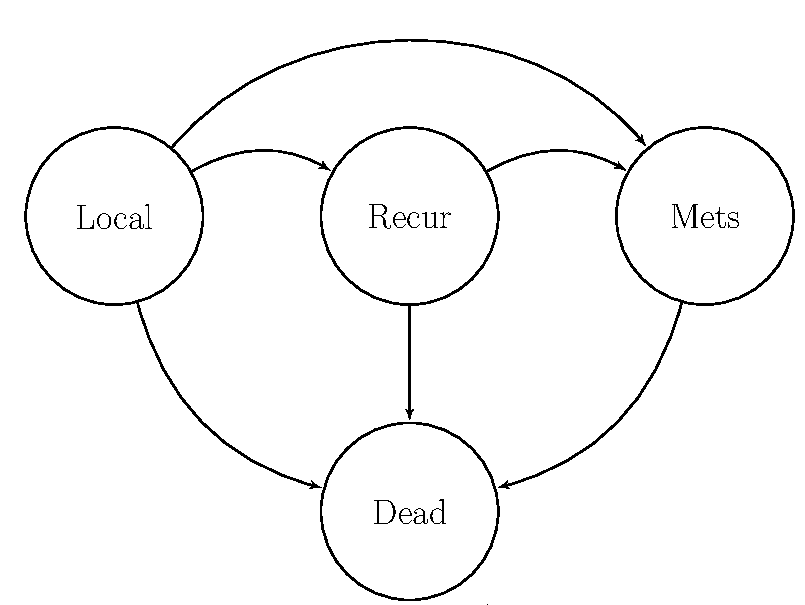
\includegraphics{figs/Markov-Diagram-BRCA} 

}

\caption{State-transition diagram of a 4-state Markov model of breast cancer.}\label{fig:state-transition-diag}
\end{figure}

The Markov model described above represents usual care for women with
breast cancer. Once we construct that Markov model, we will then add a
second strategy of a hypothetical new treatment. The effect of this new
treatment is to reduce the initial rate of cancer recurrence by 50\%;
however, the treatment also lowers the quality of life of women
(disutility of 0.05) taking the medication because of side effects.
Treatment is only taken by women who have not experienced a recurrence
(i.e., those who reside in the Local state). The Markov model for the
treatment strategy will be structurally identical to that of the usual
care strategy.

After comparing the two strategies based on quality-adjusted life
expectancy (QALE) and costs, we will incorporate costs and calculate the
incremental cost per quality-adjusted life year (QALY) gained of
treatment compared with usual care.

\section{Markov structure: Usual
care}\label{markov-structure-usual-care}

The cancer model consists of 4-states (Local, Mets, Recur, and Dead).
Therefore, we will be creating a 4x4 transition matrix. We start by
labeling the states in the transition matrix.

\begin{Shaded}
\begin{Highlighting}[]
\NormalTok{state.names <-}\StringTok{ }\KeywordTok{c}\NormalTok{(}\StringTok{"Local"}\NormalTok{, }\StringTok{"Recur"}\NormalTok{, }\StringTok{"Mets"}\NormalTok{, }\StringTok{"Dead"}\NormalTok{)}
\end{Highlighting}
\end{Shaded}

We then define the number of states in the model.

\begin{Shaded}
\begin{Highlighting}[]
\NormalTok{n.s <-}\StringTok{ }\KeywordTok{length}\NormalTok{(state.names)}
\end{Highlighting}
\end{Shaded}

From the decision problem, we know that patients in the local state face
a 2\% chance of recurrence under usual care (defined as
\texttt{p.BCA1}). Of these recurrences, 75\% will present as metastatic
disease (and patients will enter the ``Mets'' Markov state; defined as
\texttt{p.Mets1}), and the remainder present as local disease (and
patients will enter the ``Recur'' Markov state; i.e.,
\texttt{1-p.Mets1}). We will create variables to represent these
probabilities of the transition matrix. Patients in the recur state face
a 6\% chance of recurrence each year (defined as \texttt{p.BCA2}). Of
these recurrences, 90\% will present as metastatic disease (defined as
\texttt{p.Mets2}).

All patients in the local and recur state face a 0.076 annual rate of
dying from non-BCA-related causes, \(\mu_{Die}\) (defined as
\texttt{mu.Die}). Patients in the Mets state face a 0.5 anual rate of of
dying of metastatic cancer in addition to dying from other causes,
\(\mu_{DieMets}\) (defined as \texttt{mu.DieMets}).

To compute the annual probability of dying from non-BCA-related causes
(defined as \texttt{p.Die}) we transform the annual rate assuming
constant exponential rate \[
  p_{Die} = 1-exp(-\mu_{Die})
\]

The overall annual mortality rate for women with metastatic disease is
equal to the sum of the rates of dying from other causes and the excess
disease-specific mortality rate (defined as muMets). Therefore, the
annual probability of dying in the Mets state (defined as
\texttt{p.DieMets}) is converted by summing these rates and convert them
to annual probabilities

\[
  p_{DieMets} = 1-exp(-(\mu_{Die}+\mu_{DieMets}))
\]

The annual costs of breast cancer in the Local, Recur and Mets states
(\texttt{c.Local}, \texttt{c.Recur}, and \texttt{c.Mets}, respectively)
will be the same for both strategies. Table \ref{tab:param-table} shows
parameters of the model of usual care.

\begin{longtable}[]{@{}lcc@{}}
\caption{\label{tab:param-table} Table of parameters.}\tabularnewline
\toprule
\textbf{Parameter} & \textbf{R name} & \textbf{Value}\tabularnewline
\midrule
\endfirsthead
\toprule
\textbf{Parameter} & \textbf{R name} & \textbf{Value}\tabularnewline
\midrule
\endhead
Time horizon (\(n_t\)) & \texttt{n.t} & 51 years\tabularnewline
Annual discount rate (costs/QALYs) & \texttt{d.c}/\texttt{d.e} &
3\%\tabularnewline
Annual probability of recurrence & \texttt{p.BCA1} & 0.02\tabularnewline
after first local tumor diagnosis & &\tabularnewline
under usual care & &\tabularnewline
Proportion of metastatic disease & \texttt{p.Mets1} &
0.75\tabularnewline
of recurrences from the Local state & &\tabularnewline
Annual probability of recurrence & \texttt{p.BCA2} & 0.06\tabularnewline
after \textgreater{} 1 local tumor diagnoses & &\tabularnewline
Proportion of metastatic disease & \texttt{p.Mets2} &
0.90\tabularnewline
of recurrences from the Recur state & &\tabularnewline
Annual mortality & &\tabularnewline
- All-cause mortality rate & \texttt{mu.Die} & 0.08 or
age-specific\tabularnewline
- Cancer specific mortality rate & \texttt{mu.DieMets} &
0.5\tabularnewline
Annual costs & &\tabularnewline
- Cost of new treatment & \texttt{c.Rx} & 1000\tabularnewline
- Local state & \texttt{c.Local} & 500\tabularnewline
- Recur state & \texttt{c.Recur} & 5000\tabularnewline
- Mets state & \texttt{c.Mets} & 20000\tabularnewline
Utilities & &\tabularnewline
- Local state under usual care & \texttt{u.Local} & 0.95\tabularnewline
- Recur state & \texttt{u.Recur} & 0.80\tabularnewline
- Mets state & \texttt{u.Mets} & 0.40\tabularnewline
- Dead state & \texttt{u.Dead} & 0.00\tabularnewline
\bottomrule
\end{longtable}

We input the parameters as follows:

\begin{Shaded}
\begin{Highlighting}[]
\NormalTok{n.t        <-}\StringTok{ }\DecValTok{51}
\NormalTok{d.c        <-}\StringTok{ }\FloatTok{0.03}
\NormalTok{d.e        <-}\StringTok{ }\FloatTok{0.03}
\NormalTok{p.BCA1     <-}\StringTok{ }\FloatTok{0.02}
\NormalTok{p.Mets1    <-}\StringTok{ }\FloatTok{0.75}
\NormalTok{p.BCA2     <-}\StringTok{ }\FloatTok{0.06}
\NormalTok{p.Mets2    <-}\StringTok{ }\FloatTok{0.90}
\NormalTok{mu.Die     <-}\StringTok{ }\FloatTok{0.08} \CommentTok{# Mean hazard}
\NormalTok{p.Die      <-}\StringTok{ }\DecValTok{1} \OperatorTok{-}\StringTok{ }\KeywordTok{exp}\NormalTok{(}\OperatorTok{-}\NormalTok{mu.Die)}
\NormalTok{mu.DieMets <-}\StringTok{ }\FloatTok{0.5}
\NormalTok{p.DieMets  <-}\StringTok{ }\DecValTok{1} \OperatorTok{-}\StringTok{ }\KeywordTok{exp}\NormalTok{(}\OperatorTok{-}\NormalTok{(mu.Die }\OperatorTok{+}\StringTok{ }\NormalTok{mu.DieMets))}
\NormalTok{u.Local    <-}\StringTok{ }\FloatTok{0.95}
\NormalTok{u.Recur    <-}\StringTok{ }\FloatTok{0.80}
\NormalTok{u.Mets     <-}\StringTok{ }\FloatTok{0.40}
\NormalTok{u.Dead     <-}\StringTok{ }\FloatTok{0.00}
\NormalTok{c.Local    <-}\StringTok{ }\DecValTok{500}
\NormalTok{c.Recur    <-}\StringTok{ }\DecValTok{5000}
\NormalTok{c.Mets     <-}\StringTok{ }\DecValTok{20000}
\NormalTok{c.Rx       <-}\StringTok{ }\DecValTok{1000}
\end{Highlighting}
\end{Shaded}

\subsection{Transition matrix}\label{transition-matrix}

To construct the transition matrix for the usual care (UC) strategy, we
first need to define a matrix that we will name \texttt{m.P.UC}. We
initialize the matrix with \texttt{NaN} so then it can be filled with
numeric elements.

\begin{Shaded}
\begin{Highlighting}[]
\CommentTok{# Initialize matrix}
\NormalTok{m.P.UC <-}\StringTok{ }\KeywordTok{matrix}\NormalTok{(}\OtherTok{NaN}\NormalTok{, }
                 \DataTypeTok{nrow =}\NormalTok{ n.s, }\DataTypeTok{ncol =}\NormalTok{ n.s, }
                 \DataTypeTok{dimnames =} \KeywordTok{list}\NormalTok{(state.names, state.names))}
\NormalTok{m.P.UC}
\end{Highlighting}
\end{Shaded}

\begin{verbatim}
##       Local Recur Mets Dead
## Local   NaN   NaN  NaN  NaN
## Recur   NaN   NaN  NaN  NaN
## Mets    NaN   NaN  NaN  NaN
## Dead    NaN   NaN  NaN  NaN
\end{verbatim}

Each row in \texttt{m.P.UC} represent a health state and each of its
elements store the transition probbailities from that particular state.
We need to manually store each of these transition probabilities into
the matrix.

\begin{Shaded}
\begin{Highlighting}[]
\CommentTok{# Fill in matrix}
\CommentTok{# From Local}
\NormalTok{m.P.UC[}\StringTok{"Local"}\NormalTok{, }\StringTok{"Local"}\NormalTok{] <-}\StringTok{ }\NormalTok{(}\DecValTok{1} \OperatorTok{-}\StringTok{ }\NormalTok{p.Die) }\OperatorTok{*}\StringTok{ }\NormalTok{(}\DecValTok{1} \OperatorTok{-}\StringTok{ }\NormalTok{p.BCA1)}
\NormalTok{m.P.UC[}\StringTok{"Local"}\NormalTok{, }\StringTok{"Recur"}\NormalTok{] <-}\StringTok{ }\NormalTok{(}\DecValTok{1} \OperatorTok{-}\StringTok{ }\NormalTok{p.Die) }\OperatorTok{*}\StringTok{ }\NormalTok{p.BCA1 }\OperatorTok{*}\StringTok{ }\NormalTok{(}\DecValTok{1} \OperatorTok{-}\StringTok{ }\NormalTok{p.Mets1) }
\NormalTok{m.P.UC[}\StringTok{"Local"}\NormalTok{, }\StringTok{"Mets"}\NormalTok{]  <-}\StringTok{ }\NormalTok{(}\DecValTok{1} \OperatorTok{-}\StringTok{ }\NormalTok{p.Die) }\OperatorTok{*}\StringTok{ }\NormalTok{p.BCA1 }\OperatorTok{*}\StringTok{ }\NormalTok{p.Mets1}
\NormalTok{m.P.UC[}\StringTok{"Local"}\NormalTok{, }\StringTok{"Dead"}\NormalTok{]  <-}\StringTok{ }\NormalTok{p.Die}
\CommentTok{# From Recur}
\NormalTok{m.P.UC[}\StringTok{"Recur"}\NormalTok{, }\StringTok{"Local"}\NormalTok{] <-}\StringTok{ }\DecValTok{0}
\NormalTok{m.P.UC[}\StringTok{"Recur"}\NormalTok{, }\StringTok{"Recur"}\NormalTok{] <-}\StringTok{ }\NormalTok{(}\DecValTok{1} \OperatorTok{-}\StringTok{ }\NormalTok{p.Die) }\OperatorTok{*}\StringTok{ }\NormalTok{((}\DecValTok{1} \OperatorTok{-}\StringTok{ }\NormalTok{p.BCA2) }\OperatorTok{+}\StringTok{ }\NormalTok{(p.BCA2 }\OperatorTok{*}\StringTok{ }\NormalTok{(}\DecValTok{1} \OperatorTok{-}\StringTok{ }\NormalTok{p.Mets2)))}
\NormalTok{m.P.UC[}\StringTok{"Recur"}\NormalTok{, }\StringTok{"Mets"}\NormalTok{]  <-}\StringTok{ }\NormalTok{(}\DecValTok{1}\OperatorTok{-}\NormalTok{p.Die)}\OperatorTok{*}\NormalTok{p.BCA2}\OperatorTok{*}\NormalTok{p.Mets2}
\NormalTok{m.P.UC[}\StringTok{"Recur"}\NormalTok{, }\StringTok{"Dead"}\NormalTok{]  <-}\StringTok{ }\NormalTok{p.Die}
\CommentTok{# From Mets}
\NormalTok{m.P.UC[}\StringTok{"Mets"}\NormalTok{, }\StringTok{"Local"}\NormalTok{]  <-}\StringTok{ }\DecValTok{0}
\NormalTok{m.P.UC[}\StringTok{"Mets"}\NormalTok{, }\StringTok{"Recur"}\NormalTok{]  <-}\StringTok{ }\DecValTok{0}
\NormalTok{m.P.UC[}\StringTok{"Mets"}\NormalTok{, }\StringTok{"Mets"}\NormalTok{]   <-}\StringTok{ }\DecValTok{1} \OperatorTok{-}\StringTok{ }\NormalTok{p.DieMets}
\NormalTok{m.P.UC[}\StringTok{"Mets"}\NormalTok{, }\StringTok{"Dead"}\NormalTok{]   <-}\StringTok{ }\NormalTok{p.DieMets}
\CommentTok{# From Dead}
\NormalTok{m.P.UC[}\StringTok{"Dead"}\NormalTok{, }\StringTok{"Local"}\NormalTok{]  <-}\StringTok{ }\DecValTok{0}
\NormalTok{m.P.UC[}\StringTok{"Dead"}\NormalTok{, }\StringTok{"Recur"}\NormalTok{]  <-}\StringTok{ }\DecValTok{0}
\NormalTok{m.P.UC[}\StringTok{"Dead"}\NormalTok{, }\StringTok{"Mets"}\NormalTok{]   <-}\StringTok{ }\DecValTok{0}
\NormalTok{m.P.UC[}\StringTok{"Dead"}\NormalTok{, }\StringTok{"Dead"}\NormalTok{]   <-}\StringTok{ }\DecValTok{1}

\NormalTok{m.P.UC}
\end{Highlighting}
\end{Shaded}

\begin{verbatim}
##          Local       Recur       Mets       Dead
## Local 0.904654 0.004615582 0.01384675 0.07688365
## Recur 0.000000 0.873268064 0.04984828 0.07688365
## Mets  0.000000 0.000000000 0.55989837 0.44010163
## Dead  0.000000 0.000000000 0.00000000 1.00000000
\end{verbatim}

We assume that all women start in the Local state, therefore the initial
state vector defined as `s0'

\begin{Shaded}
\begin{Highlighting}[]
\NormalTok{s0 <-}\StringTok{ }\KeywordTok{c}\NormalTok{(}\DecValTok{1}\NormalTok{, }\DecValTok{0}\NormalTok{, }\DecValTok{0}\NormalTok{, }\DecValTok{0}\NormalTok{) }\CommentTok{# Everyone starts in the local state}
\end{Highlighting}
\end{Shaded}

\subsection{Run Markov model}\label{run-markov-model}

All of the components necessary to run the Markov model are now in
place. We use the function \texttt{CalculateMarkovTrace} from the
\texttt{dampack} package to run the model. The function requires a
transition probability matrix, \texttt{m.P.UC}, in this case, the
initial state vector (\texttt{s0}), and the number of cycles we want the
model to run, \texttt{n.t}. The function produces a list with the cohort
trace and the transition array, which we will call \texttt{m.Markov.UC}
for the UC strategy.

\begin{Shaded}
\begin{Highlighting}[]
\NormalTok{l.Markov.UC <-}\StringTok{ }\KeywordTok{CalculateMarkovTrace}\NormalTok{(}\DataTypeTok{M =}\NormalTok{ m.P.UC, }\DataTypeTok{p0 =}\NormalTok{ s0, }\DataTypeTok{n.cycles =}\NormalTok{ n.t)}
\end{Highlighting}
\end{Shaded}

\subsection{Rewards matrices}\label{rewards-matrices}

To calculate life years, quality adjusted life years, and cost, we will
specify a reward matrix for each of these outcomes. The elements of each
of the columns of these matrices must contain the state rewards of the
health state corresponding to that column.

For the life years, for each year spent in any of the non-dead states,
the cohort will get one year of life. That is, the elements of all the
columns corresponding non-dead states equal to one.

\begin{Shaded}
\begin{Highlighting}[]
\NormalTok{m.LY.UC <-}\StringTok{ }\KeywordTok{matrix}\NormalTok{(}\KeywordTok{rep}\NormalTok{(}\KeywordTok{c}\NormalTok{(}\DecValTok{1}\NormalTok{, }\DecValTok{1}\NormalTok{, }\DecValTok{1}\NormalTok{, }\DecValTok{0}\NormalTok{), (n.s}\OperatorTok{-}\DecValTok{1}\NormalTok{)), }
                  \DataTypeTok{byrow =} \OtherTok{TRUE}\NormalTok{,}
                  \DataTypeTok{nrow =}\NormalTok{ n.s, }\DataTypeTok{ncol =}\NormalTok{ n.s, }
                  \DataTypeTok{dimnames =} \KeywordTok{list}\NormalTok{(state.names, state.names))}
\NormalTok{m.LY.UC}
\end{Highlighting}
\end{Shaded}

\begin{verbatim}
##       Local Recur Mets Dead
## Local     1     1    1    0
## Recur     1     1    1    0
## Mets      1     1    1    0
## Dead      1     1    1    0
\end{verbatim}

For the QALY, we follow the similar procedure for the LY's reward matrix
but now each column has the utilities that correspond with that
particular state

\begin{Shaded}
\begin{Highlighting}[]
\NormalTok{m.QALY.UC <-}\StringTok{ }\KeywordTok{matrix}\NormalTok{(}\KeywordTok{rep}\NormalTok{(}\KeywordTok{c}\NormalTok{(u.Local, u.Recur, u.Mets, u.Dead), n.s),}
                    \DataTypeTok{byrow =} \OtherTok{TRUE}\NormalTok{,}
                 \DataTypeTok{nrow =}\NormalTok{ n.s, }\DataTypeTok{ncol =}\NormalTok{ n.s, }
                 \DataTypeTok{dimnames =} \KeywordTok{list}\NormalTok{(state.names, state.names))}
\NormalTok{m.QALY.UC}
\end{Highlighting}
\end{Shaded}

\begin{verbatim}
##       Local Recur Mets Dead
## Local  0.95   0.8  0.4    0
## Recur  0.95   0.8  0.4    0
## Mets   0.95   0.8  0.4    0
## Dead   0.95   0.8  0.4    0
\end{verbatim}

\begin{Shaded}
\begin{Highlighting}[]
\NormalTok{m.C.UC <-}\StringTok{ }\KeywordTok{matrix}\NormalTok{(}\KeywordTok{rep}\NormalTok{(}\KeywordTok{c}\NormalTok{(c.Local, c.Recur, c.Mets, }\DecValTok{0}\NormalTok{), n.s),}
                 \DataTypeTok{byrow =} \OtherTok{TRUE}\NormalTok{,}
                 \DataTypeTok{nrow =}\NormalTok{ n.s, }\DataTypeTok{ncol =}\NormalTok{ n.s, }
                 \DataTypeTok{dimnames =} \KeywordTok{list}\NormalTok{(state.names, state.names))}
\NormalTok{m.C.UC}
\end{Highlighting}
\end{Shaded}

\begin{verbatim}
##       Local Recur  Mets Dead
## Local   500  5000 20000    0
## Recur   500  5000 20000    0
## Mets    500  5000 20000    0
## Dead    500  5000 20000    0
\end{verbatim}

\subsection{Compute expected values}\label{compute-expected-values}

Using the \texttt{ExpectedValue} function from the \texttt{dampack}
package, we calculate the expected life years of the Markov cohort under
usual care. In the expected value function we input the transition array
(generated from the \texttt{CalculateMarkovTrace} function), the reward
matrix for life years \texttt{m.LY.UC}, discount rate \texttt{d.e} and
ask to conduct a half cycle correction.

\begin{Shaded}
\begin{Highlighting}[]
\NormalTok{ev.LY.UC <-}\StringTok{ }\KeywordTok{ExpectedValue}\NormalTok{(}\DataTypeTok{trans =}\NormalTok{ l.Markov.UC}\OperatorTok{$}\NormalTok{trans, }
                          \DataTypeTok{rwd =}\NormalTok{ m.LY.UC, }
                          \DataTypeTok{r =}\NormalTok{ d.e, }\DataTypeTok{half =}\NormalTok{ T)}
\NormalTok{ev.LY.UC}
\end{Highlighting}
\end{Shaded}

\begin{verbatim}
## [1] 8.213022
\end{verbatim}

To compute the expected QALYs, we follow the same procedure but now
using the reward matrix for QALYs \texttt{m.QALY.UC}

\begin{Shaded}
\begin{Highlighting}[]
\NormalTok{ev.QALY.UC <-}\StringTok{ }\KeywordTok{ExpectedValue}\NormalTok{(}\DataTypeTok{trans =}\NormalTok{ l.Markov.UC}\OperatorTok{$}\NormalTok{trans, }
                            \DataTypeTok{rwd =}\NormalTok{ m.QALY.UC, }
                            \DataTypeTok{r =}\NormalTok{ d.e, }\DataTypeTok{half =}\NormalTok{ T)}
\NormalTok{ev.QALY.UC}
\end{Highlighting}
\end{Shaded}

\begin{verbatim}
## [1] 7.61944
\end{verbatim}

To compute the expected costs, we follow the same procedure but now
using the reward matrix for costs \texttt{m.C.UC}

\begin{Shaded}
\begin{Highlighting}[]
\NormalTok{ev.C.UC <-}\StringTok{ }\KeywordTok{ExpectedValue}\NormalTok{(}\DataTypeTok{trans =}\NormalTok{ l.Markov.UC}\OperatorTok{$}\NormalTok{trans, }
                         \DataTypeTok{rwd =}\NormalTok{ m.C.UC, }
                         \DataTypeTok{r =}\NormalTok{ d.c, }\DataTypeTok{half =}\NormalTok{ T)}
\NormalTok{ev.C.UC}
\end{Highlighting}
\end{Shaded}

\begin{verbatim}
## [1] 10395.49
\end{verbatim}

\section{Markov structure: New
treatment}\label{markov-structure-new-treatment}

We will now model the effect of a hypothetical new treatment. This new
treatment competes with usual care. From the decision problem, we know
that the treatment is only taken by women who have not experienced a
recurrence (i.e., those who reside in the Local state).

The new treatment reduces the initial rate of cancer recurrence by 50\%
(i.e., a hazard ratio or recurrence under new treatment, defined as
\texttt{hr.Recur}). To compute the probability of cancer recurrence
associated with treatment (defined as \texttt{p.BCA1.Rx}), we first
transform the probability of cancer recurrence without treatment to a
rate. We then multiply the rate of cancer recurrence without treatment
by the treatment effect (\texttt{hr.Recur} = 0.50). Finally, we convert
the rate back to a probability to represent the probability of cancer
recurrence for those who receive treatment.

\begin{Shaded}
\begin{Highlighting}[]
\NormalTok{hr.Recur   <-}\StringTok{ }\FloatTok{0.5}
\NormalTok{p.BCA1.Rx  <-}\StringTok{ }\DecValTok{1}\OperatorTok{-}\KeywordTok{exp}\NormalTok{(}\KeywordTok{log}\NormalTok{(}\DecValTok{1}\OperatorTok{-}\NormalTok{p.BCA1)}\OperatorTok{*}\NormalTok{hr.Recur)}
\end{Highlighting}
\end{Shaded}

\subsection{Transition matrix}\label{transition-matrix-1}

We will incorporate the effects of treatment in a new transition matrix
(defined as \texttt{m.P.Rx}). The treatment transition matrix will
incorporate the treatment effects which impact transitions from the
local disease state to the disease recurrence state and from the local
disease state to the metastatic disease state. All other transitions in
the model are identical to those in the usual care transition matrix
(Table \ref{tab:param-table}).

As before, each row in the transition matrix represents a health state
and each element of the matrix store the transition probabilities.
Ultimately, we will be able to compare the expected outcomes between the
usual care and treatment models. We manually enter the transition
probabilities into the matrix.

\begin{Shaded}
\begin{Highlighting}[]
\CommentTok{# Initialize matrix}
\NormalTok{m.P.Rx <-}\StringTok{ }\KeywordTok{matrix}\NormalTok{(}\OtherTok{NaN}\NormalTok{, }
                 \DataTypeTok{nrow =}\NormalTok{ n.s, }\DataTypeTok{ncol =}\NormalTok{ n.s, }
                 \DataTypeTok{dimnames =} \KeywordTok{list}\NormalTok{(state.names, state.names))}
\NormalTok{m.P.Rx}
\end{Highlighting}
\end{Shaded}

\begin{verbatim}
##       Local Recur Mets Dead
## Local   NaN   NaN  NaN  NaN
## Recur   NaN   NaN  NaN  NaN
## Mets    NaN   NaN  NaN  NaN
## Dead    NaN   NaN  NaN  NaN
\end{verbatim}

\begin{Shaded}
\begin{Highlighting}[]
\CommentTok{# Fill in matrix}
\CommentTok{# From Local}
\NormalTok{m.P.Rx[}\StringTok{"Local"}\NormalTok{, }\StringTok{"Local"}\NormalTok{] <-}\StringTok{ }\NormalTok{(}\DecValTok{1} \OperatorTok{-}\StringTok{ }\NormalTok{p.Die) }\OperatorTok{*}\StringTok{ }\NormalTok{(}\DecValTok{1} \OperatorTok{-}\StringTok{ }\NormalTok{p.BCA1.Rx)}
\NormalTok{m.P.Rx[}\StringTok{"Local"}\NormalTok{, }\StringTok{"Recur"}\NormalTok{] <-}\StringTok{ }\NormalTok{(}\DecValTok{1} \OperatorTok{-}\StringTok{ }\NormalTok{p.Die) }\OperatorTok{*}\StringTok{ }\NormalTok{p.BCA1.Rx }\OperatorTok{*}\StringTok{ }\NormalTok{(}\DecValTok{1} \OperatorTok{-}\StringTok{ }\NormalTok{p.Mets1) }
\NormalTok{m.P.Rx[}\StringTok{"Local"}\NormalTok{, }\StringTok{"Mets"}\NormalTok{]  <-}\StringTok{ }\NormalTok{(}\DecValTok{1} \OperatorTok{-}\StringTok{ }\NormalTok{p.Die) }\OperatorTok{*}\StringTok{ }\NormalTok{p.BCA1.Rx }\OperatorTok{*}\StringTok{ }\NormalTok{p.Mets1}
\NormalTok{m.P.Rx[}\StringTok{"Local"}\NormalTok{, }\StringTok{"Dead"}\NormalTok{]  <-}\StringTok{ }\NormalTok{p.Die}
\CommentTok{# From Recur}
\NormalTok{m.P.Rx[}\StringTok{"Recur"}\NormalTok{, }\StringTok{"Local"}\NormalTok{] <-}\StringTok{ }\DecValTok{0}
\NormalTok{m.P.Rx[}\StringTok{"Recur"}\NormalTok{, }\StringTok{"Recur"}\NormalTok{] <-}\StringTok{ }\NormalTok{(}\DecValTok{1} \OperatorTok{-}\StringTok{ }\NormalTok{p.Die) }\OperatorTok{*}\StringTok{ }\NormalTok{((}\DecValTok{1} \OperatorTok{-}\StringTok{ }\NormalTok{p.BCA2) }\OperatorTok{+}\StringTok{ }\NormalTok{(p.BCA2 }\OperatorTok{*}\StringTok{ }\NormalTok{(}\DecValTok{1} \OperatorTok{-}\StringTok{ }\NormalTok{p.Mets2)))}
\NormalTok{m.P.Rx[}\StringTok{"Recur"}\NormalTok{, }\StringTok{"Mets"}\NormalTok{]  <-}\StringTok{ }\NormalTok{(}\DecValTok{1}\OperatorTok{-}\NormalTok{p.Die)}\OperatorTok{*}\NormalTok{p.BCA2}\OperatorTok{*}\NormalTok{p.Mets2}
\NormalTok{m.P.Rx[}\StringTok{"Recur"}\NormalTok{, }\StringTok{"Dead"}\NormalTok{]  <-}\StringTok{ }\NormalTok{p.Die}
\CommentTok{# From Mets}
\NormalTok{m.P.Rx[}\StringTok{"Mets"}\NormalTok{, }\StringTok{"Local"}\NormalTok{]  <-}\StringTok{ }\DecValTok{0}
\NormalTok{m.P.Rx[}\StringTok{"Mets"}\NormalTok{, }\StringTok{"Recur"}\NormalTok{]  <-}\StringTok{ }\DecValTok{0}
\NormalTok{m.P.Rx[}\StringTok{"Mets"}\NormalTok{, }\StringTok{"Mets"}\NormalTok{]   <-}\StringTok{ }\DecValTok{1} \OperatorTok{-}\StringTok{ }\NormalTok{p.DieMets}
\NormalTok{m.P.Rx[}\StringTok{"Mets"}\NormalTok{, }\StringTok{"Dead"}\NormalTok{]   <-}\StringTok{ }\NormalTok{p.DieMets}
\CommentTok{# From Dead}
\NormalTok{m.P.Rx[}\StringTok{"Dead"}\NormalTok{, }\StringTok{"Local"}\NormalTok{]  <-}\StringTok{ }\DecValTok{0}
\NormalTok{m.P.Rx[}\StringTok{"Dead"}\NormalTok{, }\StringTok{"Recur"}\NormalTok{]  <-}\StringTok{ }\DecValTok{0}
\NormalTok{m.P.Rx[}\StringTok{"Dead"}\NormalTok{, }\StringTok{"Mets"}\NormalTok{]   <-}\StringTok{ }\DecValTok{0}
\NormalTok{m.P.Rx[}\StringTok{"Dead"}\NormalTok{, }\StringTok{"Dead"}\NormalTok{]   <-}\StringTok{ }\DecValTok{1}

\NormalTok{m.P.Rx}
\end{Highlighting}
\end{Shaded}

\begin{verbatim}
##           Local       Recur       Mets       Dead
## Local 0.9138386 0.002319447 0.00695834 0.07688365
## Recur 0.0000000 0.873268064 0.04984828 0.07688365
## Mets  0.0000000 0.000000000 0.55989837 0.44010163
## Dead  0.0000000 0.000000000 0.00000000 1.00000000
\end{verbatim}

\subsection{Run Markov model}\label{run-markov-model-1}

\begin{Shaded}
\begin{Highlighting}[]
\NormalTok{l.Markov.Rx <-}\StringTok{ }\KeywordTok{CalculateMarkovTrace}\NormalTok{(}\DataTypeTok{M =}\NormalTok{ m.P.Rx, }\DataTypeTok{p0 =}\NormalTok{ s0, }\DataTypeTok{n.cycles =}\NormalTok{ n.t)}
\end{Highlighting}
\end{Shaded}

\subsection{Reward matrices}\label{reward-matrices}

The LY's reward matrix for Rx is the same than for UC.

\begin{Shaded}
\begin{Highlighting}[]
\NormalTok{m.LY.Rx <-}\StringTok{ }\NormalTok{m.LY.UC}
\end{Highlighting}
\end{Shaded}

As noted in the decision problem, treatment lowers the quality of life
(i.e., utility decrement) of women taking the medication due to side
effects (defined as \texttt{du.Local}). We incorporate the disutility
(0.05) associated with treatment into the reward matrix for the Local
state of the Rx model.

\begin{Shaded}
\begin{Highlighting}[]
\NormalTok{du.Local <-}\StringTok{ }\FloatTok{0.05}
\end{Highlighting}
\end{Shaded}

The reward matrix for Rx changes by adding the disutility from the
treatment to the Local state.

\begin{Shaded}
\begin{Highlighting}[]
\NormalTok{m.QALY.Rx <-}\StringTok{ }\KeywordTok{matrix}\NormalTok{(}\KeywordTok{rep}\NormalTok{(}\KeywordTok{c}\NormalTok{(u.Local}\OperatorTok{-}\NormalTok{du.Local, u.Recur, u.Mets, u.Dead), n.s),}
                    \DataTypeTok{byrow =} \OtherTok{TRUE}\NormalTok{,}
                 \DataTypeTok{nrow =}\NormalTok{ n.s, }\DataTypeTok{ncol =}\NormalTok{ n.s, }
                 \DataTypeTok{dimnames =} \KeywordTok{list}\NormalTok{(state.names, state.names))}
\NormalTok{m.QALY.Rx}
\end{Highlighting}
\end{Shaded}

\begin{verbatim}
##       Local Recur Mets Dead
## Local   0.9   0.8  0.4    0
## Recur   0.9   0.8  0.4    0
## Mets    0.9   0.8  0.4    0
## Dead    0.9   0.8  0.4    0
\end{verbatim}

\begin{Shaded}
\begin{Highlighting}[]
\NormalTok{m.C.Rx <-}\StringTok{ }\KeywordTok{matrix}\NormalTok{(}\KeywordTok{rep}\NormalTok{(}\KeywordTok{c}\NormalTok{(c.Local }\OperatorTok{+}\StringTok{ }\NormalTok{c.Rx, c.Recur, c.Mets, }\DecValTok{0}\NormalTok{), n.s),}
                 \DataTypeTok{byrow =} \OtherTok{TRUE}\NormalTok{,}
                 \DataTypeTok{nrow =}\NormalTok{ n.s, }\DataTypeTok{ncol =}\NormalTok{ n.s, }
                 \DataTypeTok{dimnames =} \KeywordTok{list}\NormalTok{(state.names, state.names))}
\NormalTok{m.C.Rx}
\end{Highlighting}
\end{Shaded}

\begin{verbatim}
##       Local Recur  Mets Dead
## Local  1500  5000 20000    0
## Recur  1500  5000 20000    0
## Mets   1500  5000 20000    0
## Dead   1500  5000 20000    0
\end{verbatim}

\subsection{Compute expected values}\label{compute-expected-values-1}

\begin{Shaded}
\begin{Highlighting}[]
\NormalTok{ev.LY.Rx <-}\StringTok{ }\KeywordTok{ExpectedValue}\NormalTok{(}\DataTypeTok{trans =}\NormalTok{ l.Markov.Rx}\OperatorTok{$}\NormalTok{trans, }
                          \DataTypeTok{rwd =}\NormalTok{ m.LY.Rx, }
                          \DataTypeTok{r =}\NormalTok{ d.e, }\DataTypeTok{half =}\NormalTok{ T)}
\NormalTok{ev.LY.Rx}
\end{Highlighting}
\end{Shaded}

\begin{verbatim}
## [1] 8.620571
\end{verbatim}

To compute the expected QALYs, we follow the same procedure but now
using the reward matrix for QALYs \texttt{m.QALY.Rx}

\begin{Shaded}
\begin{Highlighting}[]
\NormalTok{ev.QALY.Rx <-}\StringTok{ }\KeywordTok{ExpectedValue}\NormalTok{(}\DataTypeTok{trans =}\NormalTok{ l.Markov.Rx}\OperatorTok{$}\NormalTok{trans, }
                            \DataTypeTok{rwd =}\NormalTok{ m.QALY.Rx, }
                            \DataTypeTok{r =}\NormalTok{ d.e, }\DataTypeTok{half =}\NormalTok{ T)}
\NormalTok{ev.QALY.Rx}
\end{Highlighting}
\end{Shaded}

\begin{verbatim}
## [1] 7.673208
\end{verbatim}

To compute the expected costs, we follow the same procedure but now
using the reward matrix for costs \texttt{m.C.Rx}

\begin{Shaded}
\begin{Highlighting}[]
\NormalTok{ev.C.Rx <-}\StringTok{ }\KeywordTok{ExpectedValue}\NormalTok{(}\DataTypeTok{trans =}\NormalTok{ l.Markov.Rx}\OperatorTok{$}\NormalTok{trans, }
                         \DataTypeTok{rwd =}\NormalTok{ m.C.Rx, }
                         \DataTypeTok{r =}\NormalTok{ d.c, }\DataTypeTok{half =}\NormalTok{ T)}
\NormalTok{ev.C.Rx}
\end{Highlighting}
\end{Shaded}

\begin{verbatim}
## [1] 16061.16
\end{verbatim}

\section{Outputs}\label{outputs}

Table \ref{tab:Output} shows the outputs of the Markov model for the two
strategies.

\begin{table}[!h]

\caption{\label{tab:Output}Outcomes of Markov model by strategy}
\centering
\begin{tabular}[t]{lrrl}
\toprule
Strategy & LYs & QALYs & Costs\\
\midrule
Usual care & 8.21 & 7.62 & \$10,395.49\\
New Treatment & 8.62 & 7.67 & \$16,061.16\\
\bottomrule
\end{tabular}
\end{table}

\section{Cost-effectiveness analysis}\label{cost-effectiveness-analysis}

Finally, in Table \ref{tab:CEA}, we show the results for the CEA of the
Markov model.

\begin{table}[!h]

\caption{\label{tab:CEA}CEA of new treatment for breast cancer patients}
\centering
\begin{tabular}[t]{lrllll}
\toprule
Strategy & QALYs & Incremental.QALYs & Costs & Incremental.Costs & ICER\\
\midrule
Usual care & 7.62 & - & \$10,395.49 & - & -\\
New Treatment & 7.67 & 0.05 & \$16,061.16 & \$5,665.66 & \$105,372 /QALY\\
\bottomrule
\end{tabular}
\end{table}

\section*{References}\label{references}
\addcontentsline{toc}{section}{References}

\hypertarget{refs}{}
\hypertarget{ref-Jalal2017b}{}
Jalal, Hawre, Petros Pechlivanoglou, Eline Krijkamp, Fernando
Alarid-Escudero, Eva A. Enns, and M. G. Myriam Hunink. 2017. ``An
Overview of R in Health Decision Sciences.'' \emph{Medical Decision
Making} 37 (7): 735--46.
doi:\href{https://doi.org/10.1177/0272989X16686559}{10.1177/0272989X16686559}.


\end{document}
